\chapter{Visualising Social Contacts} % Main chapter title
\label{ch:contacts} % Change X to a consecutive number; for referencing this chapter elsewhere, use \ref{ChapterX}

After studying the about the social interaction/annotation (Chapter~\ref{ch:annotation}) and sharing data (Chapter~\ref{ch:data}), this chapter focus on how to represent social contacts through a wearable AR device. The representation of social contact varies based on their relationship with the user. A user study is conducted to test different conditions on the visual fidelity and proximity dimensions. 


% =============== PREVIOUS WORK ================

% A. Nassani, G. Lee, M. Billinghurst, T. Langlotz, and R. W. Lindeman, “Using Visual and Spatial Cues to Represent Social Contacts in Wearable AR” in SIGGRAPH ASIA 2017 Mobile Graphics and Interactive Applications. 

% =============== PREVIOUS WORK ================



\section{Proximity and Visual Fidelity}

One of the key problems with representing social networks in Augmented Reality (AR) is how to differentiate between contacts. In this paper we explore how visual and spatial cues based on social relationships can be used to represent contacts in social AR applications, making it easier to distinguish between them. Previous implementations of social AR have been mostly focusing on location based visualization with no focus on the social relationship to the user. In contrast, we explore how to visualise social relationships in mobile AR environments using proximity and visual fidelity filters. We ran a focus group to explore different options for representing social contacts in a mobile an AR application. We also conducted a user study to test a head-worn AR prototype using proximity and visual fidelity filters. We found out that filtering social contacts on wearable AR is preferred and useful.  We discuss the results of focus group and the user study, and provide insights into directions for future work.

% Rob: The abstract should give the results/findings we found in summary.
%  You should summarise the main findings in the abstract.

\begin{figure}[ht]
  \includegraphics[width=\textwidth]{images/20170618_031128_HoloLens_cropped}
  \caption{Representing social contacts in AR with different levels of proximity and visual fidelity}
  \label{fig:contacts:overview}
\end{figure}



% \section{Introduction}

% With major industry players (e.g. Microsoft, Facebook and Apple) supporting Augmented Reality (AR), it is likely that one day people will soon be using head-worn AR displays on a daily basis. One potential use for this technology could be for connecting with social networks. Just as people today use their mobile phones to connect with hundreds or thousands of "friends", wearable AR displays could be used to connect with friends and view and interact with their shared information.

% Previously, handheld and wearable AR systems have been used to view social networks in a number of different ways. For example, Presslite's Twitter 360\footnote{https://www.youtube.com/watch?v=5w7EAz8-uwU} shows virtual tweets overlaid on the real world at the locations of the people that sent them, and early versions of Junaio\footnote{https://en.wikipedia.org/wiki/Junaio} allowed people to drop virtual messages and pictures in the real world, as did the popular application Sekai Camera\footnote{https://www.youtube.com/watch?v=oxnKOQkWwF8\&t=61s}. Most of these applications were focused on asynchronous collaboration, enabling people to post virtual messages in space which can later be browsed and retrieved by other users. However similar technology could also be used for live synchronous collaboration such as a live video streaming the remote user point of view \cite{Nassani2016}, live video avatar sharing  \cite{Billinghurst2002}, or sharing realistic 3D models superimposed over the real world \cite{Fanello2016}.

% or by using virtual avatars to show a live view of remote collaborators and their surrounding space as in the Holoportation system  \cite{Fanello2016} which shows a realistic 3D AR representation of a remote collaborator.

% Tobias: Make clear here that scrolling etc is no option as we are constrained by the interactions and would require unobtrusive interactions.
% Unlike for handheld devices, by using a wearable AR display like the Microsoft HoloLens\footnote{https://www.microsoft.com/en-nz/hololens}, it could be possible to see an AR representation of the user's social network visible at all times. However, this raise the question of how to visually represent the contacts in the network. For example, if a user has a large social network with hundreds of contacts available, visually representing each of themmight clutter the user's visual space.

In our research we are interested in how to represent a social network with hundreds or thousands of contacts in a wearable AR interface. If there are dozen of virtual tags in an AR view representing people, how can they be distinguished between each other? How will this scale to hundreds or thousands of people? This is an important area of research as it will allow users to view and interact with a large number of social network followers at different levels of privacy and social engagement.

% One  of the challenges we are seeking to address is how to manage and represent communication from dozens, hundreds or thousands of contacts in a social network in an AR interface. If there are dozens of virtual tags in view representing people on the user's social network, how can they be distinguished between each other? How will this scale to hundreds or thousands of people?

% \section{Related work}

% Our work extends earlier work in representing users in Augmented and Virtual Reality (VR), social networking, and AR information filtering. Previous researchers have studied the concept of "personal space" and "social bubbles" in terms of proxemic interactions between people in different places \cite{Sousa2016}. They used floor projections and hand-held devices to communicate the presence of remote people. They also established a "gradual engagement model for remote proxmics" based on distance from the user which consists of 1) personal, 2) engaged, 3) peripheral, and 4) ambient.


% Rob: It is not good practice to use a citation as a part of speech (in this case, the subject). It is better to refer to the researchers (or the system/technique name), then give the citation. For example, "Jo [Jo et al., 2016] studied..." You should correct this throughout the paper.

% Jo \textit{et al.} studied the influence on co-presence of the background environment (AR vs VR) and the fidelity of the avatar representation of the remote user (photo-realistic vs pre-built) \cite{Jo2016}. They found that more realistic avatars had a positive impact on the feeling of co-presence between remote collaborators. Volante also studied the impact of visual appearance of avatars (realistic vs. stylized) on inter-personal emotional response of participants \cite{Volante2016}. They also found that more visual realism has lower negative effects.

% Fuchs \textit{et al.} studied telepresence via scanned 3D environment to enable social connections with people, and simulated a face-to-face interactions \cite{Fuchs2014}. The remote person was scanned and reconstructed live to the local environment. Their forecast is that 3D telepresence is going to be more popular when technology is more capable.

% Researchers  have been investigating social aspects of multi-user VR environment. %\cite{Ducheneaut2006} studied massive multiplier online games in terms of social activities, and  found that while users may prefer to be with other players, they don't necessarily like actively interacting with them. This led us to thinking that users may want to have the sense of the presence of social contacts around them, but not necessarily interact with them.

% \cite{Harris2009} studied the social behaviour of users of Second Life, and they found that users become less active over time and go to familiar places rather than being explorative and actively teleporting/flying. This suggests that people prefer routine and to be surrounded by familiar faces/places over time, forming social group.

% Some companies (such as High Fidelity\footnote{https://highfidelity.com/} and Itsme3D\footnote{https://www.itsme3d.com/}) are building social VR experiences in which people are represented as 3D virtual avatars.
% mark: [you should about how they handle crowds or if everyone is just represented the same] 
% However, there has been very little research into social representation in AR. The AR space is more challenging in terms of finding the best locations to fit avatars in the real world so they don't interfere with physical objects or appear suspended in mid-air. However, a social  AR application can also allow people to see their friends while doing other tasks; users don't have into switch to an immersive VR environment to see their social contacts.

% Researchers have also explored different ways of managing a large amount of information tags in AR interfaces.  Julier et al. showed how environmental cues such as distance, and user context can be used to filter AR content into the most relevant information \cite{Julier2002}. Hollerer et al. describe how view management techniques can be used to ensure that virtual objects can be easily seen in collaborative AR interfaces \cite{Hollerer2001}. Similarly Grasset et al. show how an image-based approach can be used to ensure AR information tags don't overlap in handheld AR \cite{Grasset2012}. 

% Previous research has explored how to filter information tags in AR interfaces based on user preferences [ref] and [ref], or even automatically based on context [To et al. 2016]. 
% mark: [Add more here]

% This previous research shows that visual fidelity can be used to distinguish between virtual avatars. Different visual representations and spatial cues can also be used to distinguish between information tags in an AR interface. However there has been little or no research on how to manage social network representations in AR for large numbers of connections. In the next section, we show how visual and proximity cues could be used to organize contacts in a wearable social AR interface.

% Allowing users to view and interact with a large number of social contacts requires filtering and categorizing information.  One way to filter/categorize contacts could be to arrange them along a social continuum, depending on how close they are to the user. For example, grouping people into Intimate Family, Friends, Colleagues and Strangers (see table \ref{tbl:visual-fidelity-proximity}), or more categories. These categories could then be shown using different levels of visual fidelity and proximity, enabling the user to easily tell the difference between people in their social network.

% \begin{table}
% 	\centering
% 	\caption{Using Visual Fidelity and Proximity to Categorise Friends}
% 	\label{tbl:visual-fidelity-proximity}
% 	\begin{tabular}{|l|l|l|}
% 		\hline
% 		\textbf{Category} & \textbf{Visual Fidelity} & \textbf{Proximity}       \\ \hline
% 		Intimate          & 3D avatar 				 & \textless1m, same space  \\ \hline
% 		Close friend      & 2D avatar                & 1-5m, close              \\ \hline
%         Acquaintance      & Bust image			 & 5-20m, nearby            \\ \hline
% 		Stranger          & Emoji			         & \textgreater20m, distant \\ \hline
% 	\end{tabular}
% \end{table}


In terms of visual fidelity, the representations of people in each of these categories could be increasingly more realistic as the categories change from Stranger to Intimate Family 
% (see figure \ref{fig:contacts:visual-fidelity-continuum}). 
For example, a user may see their spouse as a realistic virtual human superimposed over the real world, but a distant acquaintance would be a simple icon.
% \begin{figure}[ht]
% 	\centering
% 	\includegraphics[width=3in]{images/writing-images-07.eps}
% 	\caption{Changing visual fidelity over social continuum}
% 	\label{fig:contacts:visual-fidelity-continuum}
% \end{figure}
In terms of proximity, previous studies have shown that the distance between people in social settings varies according to their level of closeness \cite{Anslow2016}. We can use this to place the virtual representations of people in the real world around the user. The people that are intimate family and friends could be shown as visually closer to the user, while people who are strangers would be shown further away (see figure \ref{fig:contacts:proximic-circles}). This could be done using a body-centric virtual information space that travels with the user when they move.

The combination of using visual fidelity and proximity to categorize people from a user's social network would make it significantly easier for them to pay attention to the people that they want to. For example close friends would be represented as life-like virtual avatars near to the user, and so easily distinguished from strangers that are emoji icons further away.

\begin{figure}[ht]
  \centering
  \includegraphics[width=3in]{images/writing-images-11.eps}
  \caption{Proxemic \& Visual Fidelity Filtering of Avatars}
	\label{fig:contacts:proximic-circles}
\end{figure}

% Mark: You could move this to the future work section in the conclusion
% Other cues could be explored as well, such as placing people closer to the centre of the visual field who are more important/active, using colour to distinguish which users are currently available, or providing spatial audio cues to guide a person's attention.


\subsection{Implementation}

Using the social continuum metaphor from the previous section, we developed a prototype on the HoloLens to represent a user's social contacts in an AR environment. 
The prototype was built using Unity3D\footnote{https://unity3d.com/} 5.6 and HoloToolkit-Unity\footnote{https://github.com/Microsoft/HoloToolkit-Unity}, and the 3D avatars are from Morph3D\footnote{https://www.morph3d.com/}. 

% shows an overview of the system components. The scenario manager control the condition of the experiment, while the Friends Manager controls how friends are rendered. The Circle manager controls initial placing of the circles around the user. Spatial mapping is used to place circles and social contacts on the floor. Morph3D is used for rendering 3D avatars.

The prototype (figure \ref{fig:contacts:system-diagram}) uses the HoloLens Spatial Mapping feature to place virtual concentric circles (Circle Manager) on the ground around the user's initial position. On these circles, the social contacts are represented (Friend Manager) by either: a generic person silhouette, a 3D avatar, a 2D image, a bust image, or an emoji. The Scenario Manager controls the application, while the Friends Manager controls how friends are rendered. The Circle Manager controls initial placing of the circles around the user. Spatial Mapping is used to place circles and social contacts on the floor. Figure 1 shows the AR view of the user's social network.


\begin{figure}[ht]
  \centering
  \includegraphics[width=3in]{images/system-diagram.eps}
  \caption{System components}
	\label{fig:contacts:system-diagram}
\end{figure}


% mark: It would be good to have a figure showing the AR interface

% mark: [It might be good to add more information here about the hololens interface – software used to build it in (Unity?) content used etc]

To arrange the social network, the user can use hands gestures (e.g. tap and drag) to move a virtual avatar closer or further away from the centre of the circles, changing the social group the contact belongs to, and the representation of the avatar automatically updates to match the selected social group. For instance, if the user selects a 3D avatar from the Intimate circle and moves her to the Friends circle, then her representation will turn into a bust image to reflect the destination social group.

% TODO: (Gun) Add some screen captures of the prototype implementation on HoloLens. Would be good to have the four conditions shown with this. Or is Figure 1 for this? Then you should better refer to the figure here in the text. Also would be nice to have the pictures to have a background of real environment to make it clear it is an AR visualization, rather than fully virtual.

% TODO: add system image + UI screenshot

\subsection{Focus Groups}

% Mark: You should say how many men and women there are and their ages.
To evaluate the interface concept and collect feedback from potential users, we conducted two focus group sessions with a total of 11 participants. 
The first group consisted of six post-graduate students working on AR/VR research. The second group was a mix of five professional visual graphics and user experience designers who have not worked on AR/VR before. 
Each session was divided into two activities: (1) user participatory design and (2) a usability test with the prototype. 

The focus group began with a discussion and brainstorming session on how to visualise social network contacts in an AR environment. We briefly introduced the concept of social networking in AR and the challenges observed including visual clutter, yet no demonstration of the prototype system was given to avoid priming.
This activity included three tasks: 
% \textit{Task 1}) Imagine the future of social networks in AR. \textit{Task 2}) Map social groups in terms of physical distance. \textit{Task 3}) Map social groups in terms of visual fidelity.

\begin{itemize}
	\item T1: Imagine the future of social networks in AR 
	\item T2: Map social groups in terms of physical distance 
	\item T3: Map social groups in terms of visual fidelity 
\end{itemize}


\textit{Task 1}: We asked participants to draw or describe their vision of the future of how to represent social networks in AR. They then presented their ideas to the group and exchanged feedback.

% TODO: (Gun) Any figures to show the task?

\textit{Task 2}: We asked participants to order four different social groups (Intimate, Friend, Acquaintance, Stranger) in terms of physical distance from the user. We gave them four silhouettes that had one of the social groups written on the top and asked them to place silhouettes on an arrow that has four position; closest, close, far and farthest.

\textit{Task 3}: We asked the participants to match four different types of visual fidelity (3D avatar, 2D image, Bust image, Emoji) to four social groups (Intimate, Friend, Acquaintance, Stranger). This task included two sets of avatars, one male and one female.

In the second session, the usability test, we gave a demonstration of the prototype implementation, and asked participants for feedback on the following four conditions (see Figure \ref{fig:contacts:conditions}): 

\begin{figure*}
	\centering
	\includegraphics[width=\linewidth]{images/conditions-transparent-background}
	\caption{Four conditions of representing social contacts as seen through HoloLens; Baseline (B): same distance and visual, Proximity (P): different distance, Visual Fidelity (V): different visual, and Combined (C): different distance and visual}
	\label{fig:contacts:conditions}
\end{figure*}


\textit{Baseline (B):} all avatars had the same visual representation (silhouette) and they were at the same distance away from the user.

\textit{Proximity (P):} the avatars were placed at different distances from the user based on their social intimacy (the Intimate group was the closest, then Friends, then Acquaintance, then Strangers). However, they were all a silhouette representation.

\textit{Visual Fidelity (F):} the avatars placed at the same distance but had different visual representations based on their social group. The Intimate group was represented by an animated 3D avatar that moved and looked around. Friends were represented by 2D static images. Acquaintances in 2D busts, and Strangers were emojis.

\textit{Combined (C):} used both proximity and visual fidelity to filter social connections based on their social group.

Each participant tried the four conditions in a random order and for each condition, participants filled out a System Usability Scale (SUS) questionnaire \cite{brooke1996sus}. They also answered the following three subjective questions, on a Likert scale of 1 to 7, where 1=\textit{Not very natural/easy} and 7=\textit{Very natural/easy}:

\begin{itemize}
	\item SQ1: How natural was the mapping of proximity to social relationship?
	\item SQ2: How natural was the mapping of visual fidelity to social relationship?
	\item SQ3: How easy was it to distinguish between the different avatar types?
\end{itemize}

\subsection{Results}

% mark: It would be good to talk about the two different groups – one from Uni and one from work.
We recruited 11 participants (four female, aged between 16 and 41 years old, Median=29, SD=5.89). Most (85\%) used social networks (e.g., Facebook, Instagram, Snapchat) on a daily basis, and about 60\% reported using AR/VR headsets (e.g., HoloLens, HTC Vive) on a monthly basis or more often. Only two people reported having no experience with AR/VR headsets before.

\subsection{User Participatory Design}

% The focus group consisted of three tasks in the brainstorming session: 

For \textit{task 1}, when asked about how would they imagine representing social contacts in an AR platform, there were the two main recurring themes, listed in the order of popularity.

\textit{Theme 1 - Virtual Avatars}: Display virtual avatars representing friends around the users using spatial cues to distinguish them. The user can interact with other avatars to see their interests, posts or their location. The user can initiate a voice or video call with one of their contacts by interacting with the avatars.

\textit{Theme 2 - Miniatures}: Display miniature avatars (spheres, or bubbles) spread around the user environment, each bubble representing a friend. The locations of the bubbles could be determined by the social connection that the user has with that contact. Close friends could be placed near the user on a table surface while strangers are on the ground or further away. A user could pick up one of these bubbles and move them from one social group to another. 
% The bubbles could follow the user when he moved to another place/room, and re-arrange themselves according to the physical surrounding environment.
% Mark: Only these two additional ideas?

Other themes included seeing what others are seeing from their point of view, and highlighting who is online (coloured) or offline (grayed out) were also mentioned.


% mark: [Do you have a list of all the 11 ideas? Maybe we can include that somehow]

% TODO (Gun): [Add couple of sentences here (or in the discussion section) about how similar or different were the user's proposed design compared to our own design (prototype system).]

For \textit{task 2} 
(Figure \ref{fig:contacts:visual-fidelity})
, we asked participants to order friend categories based on proximity (distance from the user). Most (90\%) participants ordered the categories as follows: Intimate, Friend, Acquaintance, Stranger on the scale from closest to furthest away from the user. This shows that users associated proximity with intimacy.

\begin{figure}[ht]
	\centering
	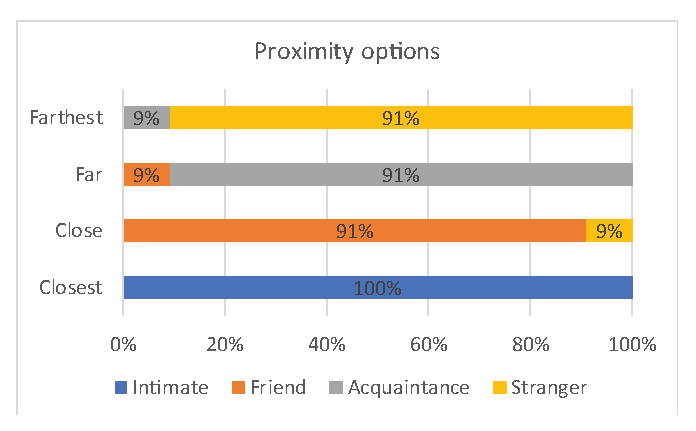
\includegraphics[width=3in]{images/analysis-images-06.eps}
	\caption{Visual fidelity categorisation for social contacts}
	\label{fig:contacts:visual-fidelity}
\end{figure}

For \textit{task 3} 
(Figure \ref{fig:contacts:proximity})
, we asked participants to categorise four types of visual fidelity. Most participants (73\%) associated 3D avatars with an Intimate relationship, 59\% marked 2D image as a  friend, 64\% associated the Bust image for Acquaintances, while 45\% marked Emoji for Strangers.
% mark: In the discussion section you might want to talk about the outliers

% mark: Maybe put this as a table?

% TODO (Gun): [Add here (or in the discussion section) how the results aligns with (or different from) our proposed design of the protype system].

% mark: [It would be good to include comments from the users as to why they organized them in this way]

\begin{figure}[ht]
	\centering
	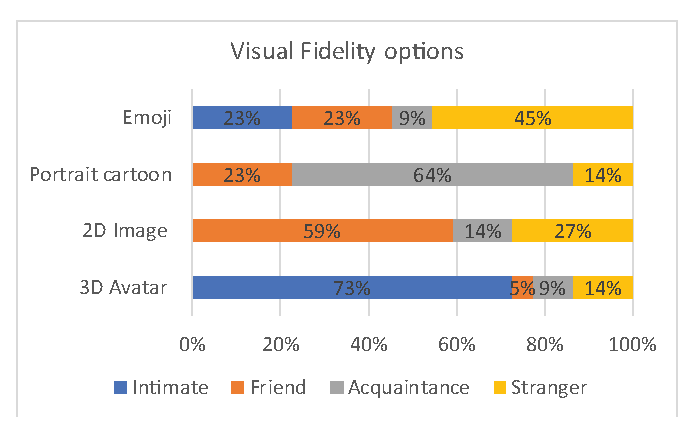
\includegraphics[width=3in]{images/analysis-images-01.eps}
	\caption{Proximity categorisation for social contacts}
	\label{fig:contacts:proximity}
\end{figure}

\subsection{Usability}

% \begin{figure}[ht]
% 	\centering
% 	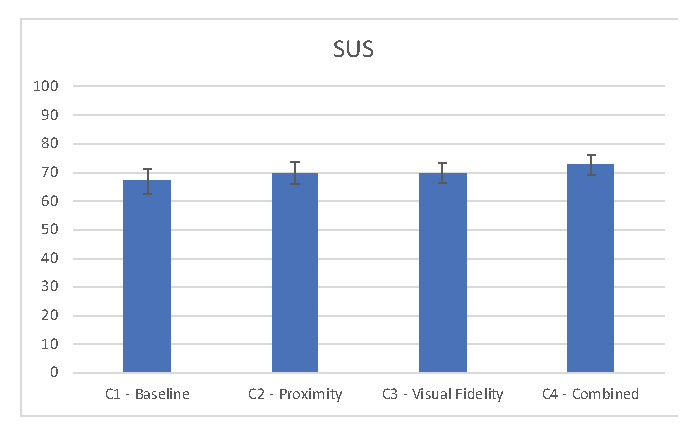
\includegraphics[width=3in]{images/analysis-images-02.eps}
% 	\caption{System Usability Score. Whiskers indicate standard error.}
% 	\label{fig:contacts:sus}
% \end{figure}
% TODO (Gun): In the figure caption, you should mention what does the whiskers (error bars) represent. BTW, based on the error bars seems you might have had significant results? Any inferential statistics to report here? I would suggest running Aligned Rank Transform Repeated-measure two-way ANOVA. 
% mark: You should label them B,P,F and C
The SUS scores 
% (Figure \ref{fig:contacts:sus}) 
show conditions B (69), V (69) and C (72) are rated "Good" while B is "OK" (67). This shows a slight increase in usability in the Proximity and Visual Fidelity conditions, yet no statistically significant difference was found. 
We ran aligned rank transform on SUS results to order to run 2-way repeated measure ANOVA analysis with two factors Proximity and Visual Fidelity; 2-level each. We didn't find any significant differences in terms of SUS between Proximity and Visual Fidelity. 
% mark: Did you do a statistical test to compare between conditions? It would be good to put the results. You can say there weren't enough people if there wasn't statistical difference.

The subjective questionnaire (Figure \ref{fig:contacts:sq2}) shows an increase in how natural people felt the mapping to proximity (SQ1) was in the Proximity condition. We ran a Friedman test and found that there was a statistically significant difference in rating the four conditions, $X^2(2)=18.402,p<0.001$. Post hoc analyses with Wilcoxon signed-rank tests were conducted with a Bonferroni correction applied, resulting in a significance level set at $alpha$=0.008. There was a significant difference between C and B ($Z=-2.687, p=0.007$). However, there were no statistically significant differences between the other conditions.

Similarly, there was an increase in how natural people felt the mapping to visual fidelity (SQ2) was in the Visual Fidelity condition. We ran a Friedman test and found that there was a statistically significant difference in rating the four conditions, $X^2(2)=21.194,p<0.001$. Post hoc analyses with Wilcoxon signed-rank tests were conducted with a Bonferroni correction applied, resulting in a significance level set at $alpha$=0.008. There were significant differences between V and B  ($Z=-2.825, p=0.005$) and between C and B ($Z=-2.820, p=0.005$). However, there were no statistically significant differences between the other conditions.

As for the (SQ3), people felt it was easier to distinguish between different avatars in both the Visual Fidelity and Combined conditions. We ran a Friedman test and found that there was a statistically significant difference in rating the four conditions, $X^2(2)=20.967,p<0.001$. Post hoc analyses with Wilcoxon signed-rank tests were conducted with a Bonferroni correction applied, resulting in a significance level set at $alpha$=0.008. There were significant differences between V and B  ($Z=-2.816, p=0.005$) and between C and B ($Z=-2.829, p=0.005$). However, there were no statistically significant differences between the other conditions.


\begin{figure}[ht]
	\centering
	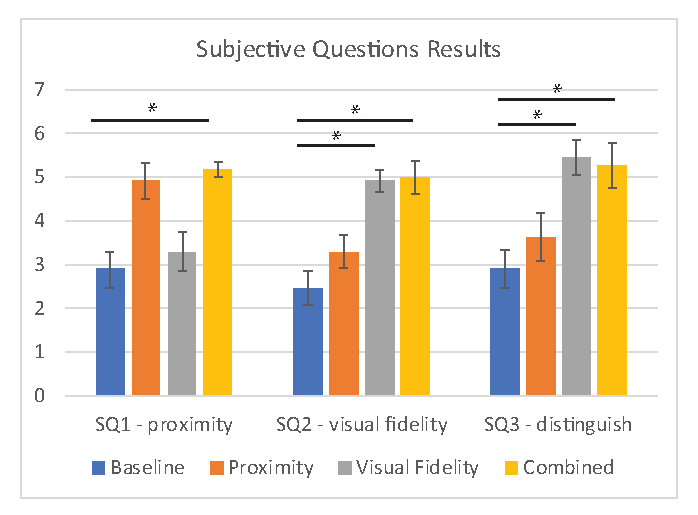
\includegraphics[width=3in]{images/analysis-images-05.eps}
	\caption{Subjective questions results by condition by question. Whiskers indicate standard error. *=statistically significant difference}
	\label{fig:contacts:sq2}
\end{figure}

% Rob: Should be: "Subject question results by condition."

For ranking the conditions 
(Figure \ref{fig:contacts:ranking})
, participants ranked the four conditions from 4 to 1 where 4 was the most preferred and 1 the least preferred. Results show that participants preferred V and C over P and B. We ran a Friedman test and found that there was a statistically significant difference in ranking the four conditions, $X^2(2)=15.222,p=0.002$. Post hoc analyses with Wilcoxon signed-rank tests were conducted with a Bonferroni correction applied, resulting in a significance level set at $alpha$=0.008. There was a significant difference between V and B  ($Z=-3.035, p=0.002$). However, there were no statistically significant differences between the other conditions.

\begin{figure}[ht]
	\centering
	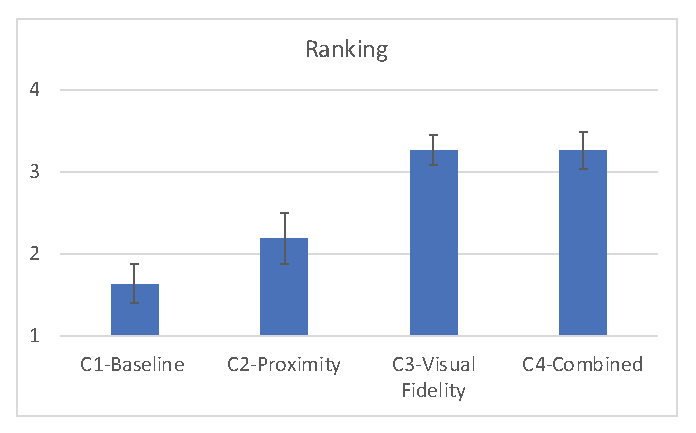
\includegraphics[width=3in]{images/analysis-images-04.eps}
	\caption{Ranking (4=highest, 1=lowest) Whiskers indicate standard error.}
	\label{fig:contacts:ranking}
\end{figure}

% Mark: If you have space it would be good to add your own observations of how people used the prototype.

\subsection{Discussion}

From the user study, we found that subjects preferred having a filter to represent their social contacts rather than no filter (i.e., Baseline condition). Based on the ranking results, the most preferred filters are the Visual Fidelity and Combined filters, followed by the Proximity filter.
% TODO (Gun) : [Discuss how this is similar to our proposed design or what are the difference? How this would affect further development/design of the social AR interface?]
The subjective questions revealed that each condition was representing the natural mapping/filter of the user's social contacts (i.e., "SQ1-how natural the proximity" scored high in "P" and so on). Participants felt that V was the easiest for distinguishing avatars.

In terms of the strengths and weaknesses of each condition, participants didn't like the Baseline condition because that they couldn't easily distinguish the avatars. For example, on participant said, "\textit{I can't distinguish avatar so well, I don't want to look around at everyone at the same distance}". This confirms our original predictions regarding the placing of social contacts.
With the Proximity condition, participants reported positive feedback and an increase in avatar presence, but were not able to fully distinguish users from each other.  One user said "\textit{I feel more spatial presence}", but another said "\textit{I need to look around more to see what is where.}"
In the Visual Fidelity condition, participants reported that it was easy to distinguish contact, but the interface could be improved. One user said "This one felt more comfortable with people at a distance and was easy to tell people apart", while another user said "Take more visual space for people whom I don't want to interact with."
In the Combined condition, participants reported it was the best because they felt that it was easier to distinguish between avatars. One user said "\textit{More info is available (fidelity + distance)..}"
% , while another said [put 100\% positive quote]   
However, some participants didn't like it when the avatars were too close and recommended increasing the minimum distance between the user and the closest circle.

Overall, the results confirmed our hypothesis that users would prefer to have their social contacts filtered out based on their relationship to them. The question is which filter (Proximity or Visual fidelity) is best for each condition. Users seems to prefer either visual fidelity of a combination of visual fidelity and proximity. This may remain a user preference. 

\subsection{Summary}

In this paper, we investigated different visualisation options for representing social contacts in a wearable AR interface. We conducted two focus groups to get feedback from potential users about how they would want to organize social contacts in an AR interface. We found that users identified visual representation and spatial cues as common ways to do this. This matched the interface metaphor used to develop a working prototype.

We tested the usability and user preference of four conditions in a prototype AR interface on a HoloLens display: 1) Baseline, 2) Proximity, 3) Visual Fidelity and 4) Combined. Participants indicated that it was useful to have some different visual fidelity representations of their AR social contacts, and that a combined use of visual fidelity and proximity was also useful.

In the future, we plan to explore and further develop visual fidelity representations of social contacts. For instance, displaying avatars as miniatures on a near-by surface. We will also investigate different ways to interact with other users in social networks who are either physically collocated or remote.


\section{Placing Social Contacts}
\label{sec:contacts:placing}

% TODO: split these 2 images
\begin{figure}
    \centering
    \includegraphics[width=5.5in]{images/images-06-cmyk.eps}
    \caption{Prototype interface of contact placement dimension. Life-size (left) on ground vs. Miniature (right) on a nearby surface.} 
    \label{fig:continuum:conditions}
\end{figure}

We implemented a prototype (Figure \ref{fig:continuum:conditions}) to test two conditions on the contact placement dimension, one viewing avatars in life-size, and the other viewing in miniature. 
We collected feedback from potential users during an open day at our lab as the participants tried demonstrations of the two conditions: C1-Life-sized (L) and C2-Miniature (M) representations of friend avatars. We collected feedback from 27 participants. On trying a demonstration of each condition, we asked participants to rate their experience on a 7-point Likert scale for three subjective questions on: 1) ease of use, 2) natural interaction, and 3) usefulness. We also asked participants to think of situations where it would be useful to use each condition. Then we asked them to choose one of the conditions as the best condition based on their experience. 

The results of the questions (Figure \ref{fig:continuum:results}) did not show any statistically significant data for this pilot study. However, we did notice a trend on Natural and Usefulness favouring the Miniature condition over the Life-size condition. A Wilcoxon signed-rank test showed that using Life-Sized or Miniature did not elicit a statistically significant change in ease of use ($Z=-.529, p=.597$), natural interaction ($Z=-1.616, p=.106$), nor usefulness ($Z=-1.664, p=0.096$). Participants reported the most useful scenarios for the Life-size condition as \enquote{face to face conversations with a social contact} or \enquote{when zooming in to a subset group of friends.} For the Miniature condition, participants reported \enquote{seeing the overall picture of social contacts} or \enquote{moving contacts between different social circles} as being useful. We also asked participants to rank the two conditions in terms of preference. Results (Figure \ref{fig:continuum:results}) show that more participants preferred the Miniature condition. A Wilcoxon signed-rank test showed that using Life-Sized or Miniature did not reach statistical significance ($Z=-.577, p=.564$).

\begin{figure}[ht]
    \centering
    \includegraphics[width=3in]{images/images-09.eps}
    \caption{\textit{Top:} average results of subjective questions grouped by condition by question. \textit{Bottom:} average ranking results of preferred condition between Life-size and Miniature; 1=most preferred, 2=least preferred. Whiskers indicate standard error.}
    \label{fig:continuum:results}
\end{figure}